%\documentclass[jkps,preprint,fleqn,showpacs,showkeys]{revtex4}
\documentclass[jkps,fleqn,showpacs,showkeys]{revtex4}
\usepackage[pdftex]{graphicx}
\usepackage{amssymb}
\usepackage[dvipsnames]{xcolor}
\usepackage{amsmath}
\usepackage{bm}
\usepackage{tabularx}


\usepackage{kotex}


\begin{document}
\newcolumntype{C}[1]{>{\centering\arraybackslash}p{#1}}


\setcounter{page}{1}
\title[]{Analysis of the near-side Ridge in pp collisions via Momentum-Kick model}
\author{Jaesung \surname{Kim}}
\author{Jin-Hee \surname{Yoon}}
\email{jinyoon@inha.ac.kr}
% \thanks{Fax: +82-2-6490-5750}
\affiliation{Department of physics, Inha University, Incheon 402-751}
\date[]{Received !Month !day 2023}

\pacs{}
\keywords{Oh My God!}


\begin{abstract}
  The near-side ridge structure was observed at the long-range in the two-particle correlations, which is observed in heavy-ion collisions like AuAu collision at the Relativistic Heavy Ion Collider (RHIC), PbPb and pPb collisions at the Large Hadron Collider(LHC).
  The ridge structure in the heavy-ion collisions could be understood by hydrodynamic models.
  However, the ridge structure is also observed in the proton-proton collision, which is a small system, in the LHC experiments.
  Since the small system creates a lower density than heavy-ion collisions, we assume that the effect of kinematics is increased.
  In this study, we invWestigate the applicability of the Momentum-Kick model.
  The Momentum-Kick model is based on kinematics, which explains the ridge structure as kicked medium partons by jet particles.
  Therefore, we expect that the Momentum-Kick model can explain proton-proton collision at 13TeV in the LHC for various momenta and multiplicity.
  And we conclude that the Momentum-Kick model makes clear the near-side ridge structure in the proton-proton collision.
\end{abstract}


\maketitle

\section*{INTRODUCTION}
\label{sec:Introduction}

The ridge structure refers to the shape of ‘ridge’ in the $\Delta\eta - \Delta\phi$ correlation, which appears at the high $\Delta\eta$ range.
Previously, the ridge structure was observed in the case of heavy-ion collisions such as AuAu collisions at the Relativistic Heavy Ion Collider (RHIC) \cite{ref12, ref13, ref14, ref15, ref16, ref17, ref18, ref19, ref20, ref21, ref22, ref23, ref24, ref25, ref26, ref27}, and PbPb at the Large Hadron Collider (LHC) \cite{ref1, ref2, ref3, ref4, ref5, ref6, ref7, ref8, ref9, ref10, ref11}.
In these cases, the ridge structure can be understood by collective motion, based on hydrodynamics theory, because it is enough to create high-temperature and high-density environment.
And this is the hint of Quark-Gluon Plasma (QGP) state.
Recently, however, the ridge structure is also observed in the high multiplicity of the proton-proton collision, which is the small system.
It was expected that the small system could not create an environment like heavy-ion collisions, and the medium doesn't make the collective motion.

The Momentum-Kick model\cite{Wong_2, Wong_3, Wong_4, Wong_5} is based on pure kinematics between near-side jet and medium partons, which assumes that the medium particles are kicked by near-side jet particles, and the kicked partons make a collective motion, like heavy-ion collision.
Since the Momentum-Kick model is successfully applying the experimental results in AuAu at 200 GeV\cite{Wong_1}, PbPb at 2.76 TeV\cite{PbPb}, and pp at 13 TeV\cite{Hanul}, we expect that the model can explain well ridge structure at the various momentum in high multiplicity small system.
We describe the various momentum in proton-proton collisions, which is a further step from the previous proton-proton at 13TeV results\cite{Hanul}, using the same $f_R \langle N_k \rangle$ form in the previous PbPb at 2.76TeV results\cite{PbPb}.
Therefore, we will analyze the high multiplicity proton-proton collision at 13 TeV from A Large Ion Collider Experiment (ALICE), Compact Muon Solenoid (CMS), and A Toroidal LHC Apparatus (ATLAS) experiments via the Momentum-Kick model\cite{alice,cms,atlas}.

\section*{Momentum-Kick Model}
\label{sec:Momentum-Kick Model}

The Momentum-Kick model describes the results of experiments at the near-side parts, through the behavior of near-side jet fragments kicking the medium partons.
The kicked medium partons make the collective motion, which is the reason for the near-side ridge structure.
Since the small systems create lower density of the medium particles, we expect that kinematics behavior is more dominant in the small system than heavy-ion collisions.
Hence, the Momentum-Kick model will be anticipated to successfully describe proton-proton collision at 13TeV in high multiplicity.


Since the near-side jet fragments usually distribute at short-range and the pp at 13TeV data have only long-range and near-side data, we use only the ridge component and it is expressed as:
\begin{equation} \label{equation:eq1}
\frac{2}{3} f_R\left\langle N_k\right\rangle \frac{dF}{p_T dp_T d\Delta\eta d\Delta\phi},
\end{equation}
where $\Delta \eta $ and $\Delta \phi$ are the differences of $\eta$ and $\phi$ between jet and the other particles, $f_R$ is the average survival factor of ridge particles, and $\left\langle N_k\right\rangle$ is the average of kicked partons per-trigger particle.

The Momentum-Kick model explains the ridge component via soft scattering model as follows:
\begin{equation} \label{equation:eq4}
\frac{dF}{p_Tdp_Td\eta d\phi}
= \left[\frac{dF}{p_{Ti}dp_{Ti}dy_id\phi_i} \frac{E}{E_i} \right]_{\mathbf{p}_i=\mathbf{p}-\mathbf{q}}\times\sqrt{1-\frac{m^2}{\left(m^2+p_T^2\right){\cosh}^2y}}.
\end{equation}
$ dF / p_{Ti}dp_{Ti}dy_id\phi_i $ is the normalized initial parton distribution, which implies the distribution before freezing out.
$\mathbf{p}_i$ is the initial parton momentum, and $\mathbf{p}$ is the momentum of the final parton after the kicked as $\mathbf{q}$.
Since the most of the near-side jet is concentrated in the perpendicular direction of beam axis, the transverse momentum of initial particles is written as follows:
\begin{equation} \label{equation:eq5}
p_{Ti}^2=p_{T}^2-2p_{T} q \cos\left(\Delta\phi\right)+q^2.
\end{equation}
% $\Delta\eta,\Delta\phi \sim 0$ region, we set $\eta_{\text{jet}}=0$.
$E/E_i$ insures conservation of energy between initial and final partons.
$\sqrt{ \left. 1- m^2 \middle/ \left(m^2+p_T^2\right){\cosh}^2y \right.}$ converts the rapidity into pseudo-rapidity.

The initial parton momentum distribution is expressed as follows:
\begin{equation} \label{equation:eq6}
\frac{dF}{p_{Ti}dp_{Ti}dy_id\phi_i}=A_{\text{ridge}}\left(1-x\right)^a\frac{e^{ \left. -\sqrt{m^2+p_{Ti}^2} \middle/ T \right. }}{\sqrt{m_d^2+p_{Ti}^2}},
\end{equation}
where $A_{\text{ridge}}$ is the normalization constant.
$T$ is one of the major parameters to explain momentum distribution, indicating the temperature of medium particles.
Since pions are expected to take up the majority of partons, we set $m$ as the mass of the pion, which $m$ means the medium parton mass.
$m_d$ is a cut-off parameter that prevents divergence at small $p_{Ti}$.
$a$ is a fall-off parameter, which determines the rate of decrease of $1-x$ distribution.
$m_d$ and $a$ are set the same as references\cite{PbPb, Wong_1}, which we take $m_d = 1.0$GeV and $a = 0.5$, for the general application of the Momentum-Kick model\cite{Wong_1}.
Also, $x$ is the light-cone variable written as follows:
\begin{equation} \label{equation:eq8}
x=\frac{\sqrt{m^2+p_{Ti}^2}}{m}e^{\left|y_i\right|-y_b},
\end{equation}
where $y_b$ is the rapidity of the beam defined as $y_b=\cosh^{-1}{\sqrt{s_\text{NN}}/2m_N}$. $m_N$ is the mass of beam particles, set as the proton mass.


\section*{FITTING RESULTS}
\label{sec:FITTING RESULTS}

\subsection{Experimental environment}
\label{subsec:Experimental environment}

We verify our model in ALICE, CMS and ATLAS experiments\cite{alice,cms,atlas} via least square method.
The conditions of the data analyzed in these experiments are summarized in Table \ref{table:range}.
In the case of $\Delta\eta$ range, ALICE experiment is narrower than CMS and ATLAS.
Moreover, ALICE experiment defines the high multiplicity as the top $0\sim0.1\%$ multiplicity, which is distinct from other experiments in that they define the range of multiplicity.
And, the ALICE and CMS experiments split their data as $p_T$ range.

\begin{table}[ht]
  \centering
  \begin{tabular}{C{3cm} | C{3cm}  C{3cm}  C{3cm} } 
  \hline \\[-1 ex]
   & ALICE\cite{alice} & CMS\cite{cms} & ATLAS\cite{atlas} \\ [1 ex] \hline\hline \\[-1.5ex]
  $\Delta \eta $ range & $1.6<|\Delta \eta |<1.8$ & $2<|\Delta \eta |<4$ & $2<|\Delta \eta |<5$ \\ [1ex] 
  Multiplicity & $0\sim0.1\%$ & $N_{\text{trk}}^{\text{offline}} \geq 105$ & $N_{\text{ch}}^{\text{rec}} \geq 90$ \\[1ex] 
  $p_T$ range & $1<p_T<4$ & $0.1<p_T<4$ & $0.5<p_T<5$ \\[1 ex]
  \hline
 \end{tabular}
 \caption{The experimental environment in ALICE, CMS, and ATLAS data \cite{alice, cms, atlas}}
 \label{table:range}
\end{table}

All three results used different analyzing methods, the ALICE and CMS analysis used Zero Yield At Minimum (ZYAM) method, a traditional experimental analysis method.
In this method, the minimum value is set to zero by subtracting.
However, ATLAS used the peripheral subtraction method.
It takes the ridge component from the experiment data by subtracting the peripheral component, which is low multiplicity pp collisions, to check the flow effect.
The Momentum-Kick model has applied the ZYAM method's results, we apply ZYAM method when we use ATLAS experiment data for consistency.

\subsection{Does $f_R\langle N_k \rangle$ have $p_T$ dependence?}
\label{subsec: pT depnedence}

Since the initial parton momentum distribution is normalized, $f_R\langle N_k \rangle$ describes the number of particles, which $f_R$ means the survival ratio of initial partons and $\langle N_k \rangle$ is the number of kicked medium partons.
Therefore, we can assume that $f_R\langle N_k \rangle$ has $p_T$ dependence.
This assumption was already introduced in paper\cite{PbPb}, and the paper successfully explained the PbPb at 2.76 TeV results.
Hence, we need to check whether this assumption applies to proton-proton collisions.
Following figure is the fitting results of $f_R\langle N_k \rangle$.
We can find the difference between $Ae^{-{B} / p_T -C p_{T}}$ and constant.

\begin{figure}[ht]
\centering
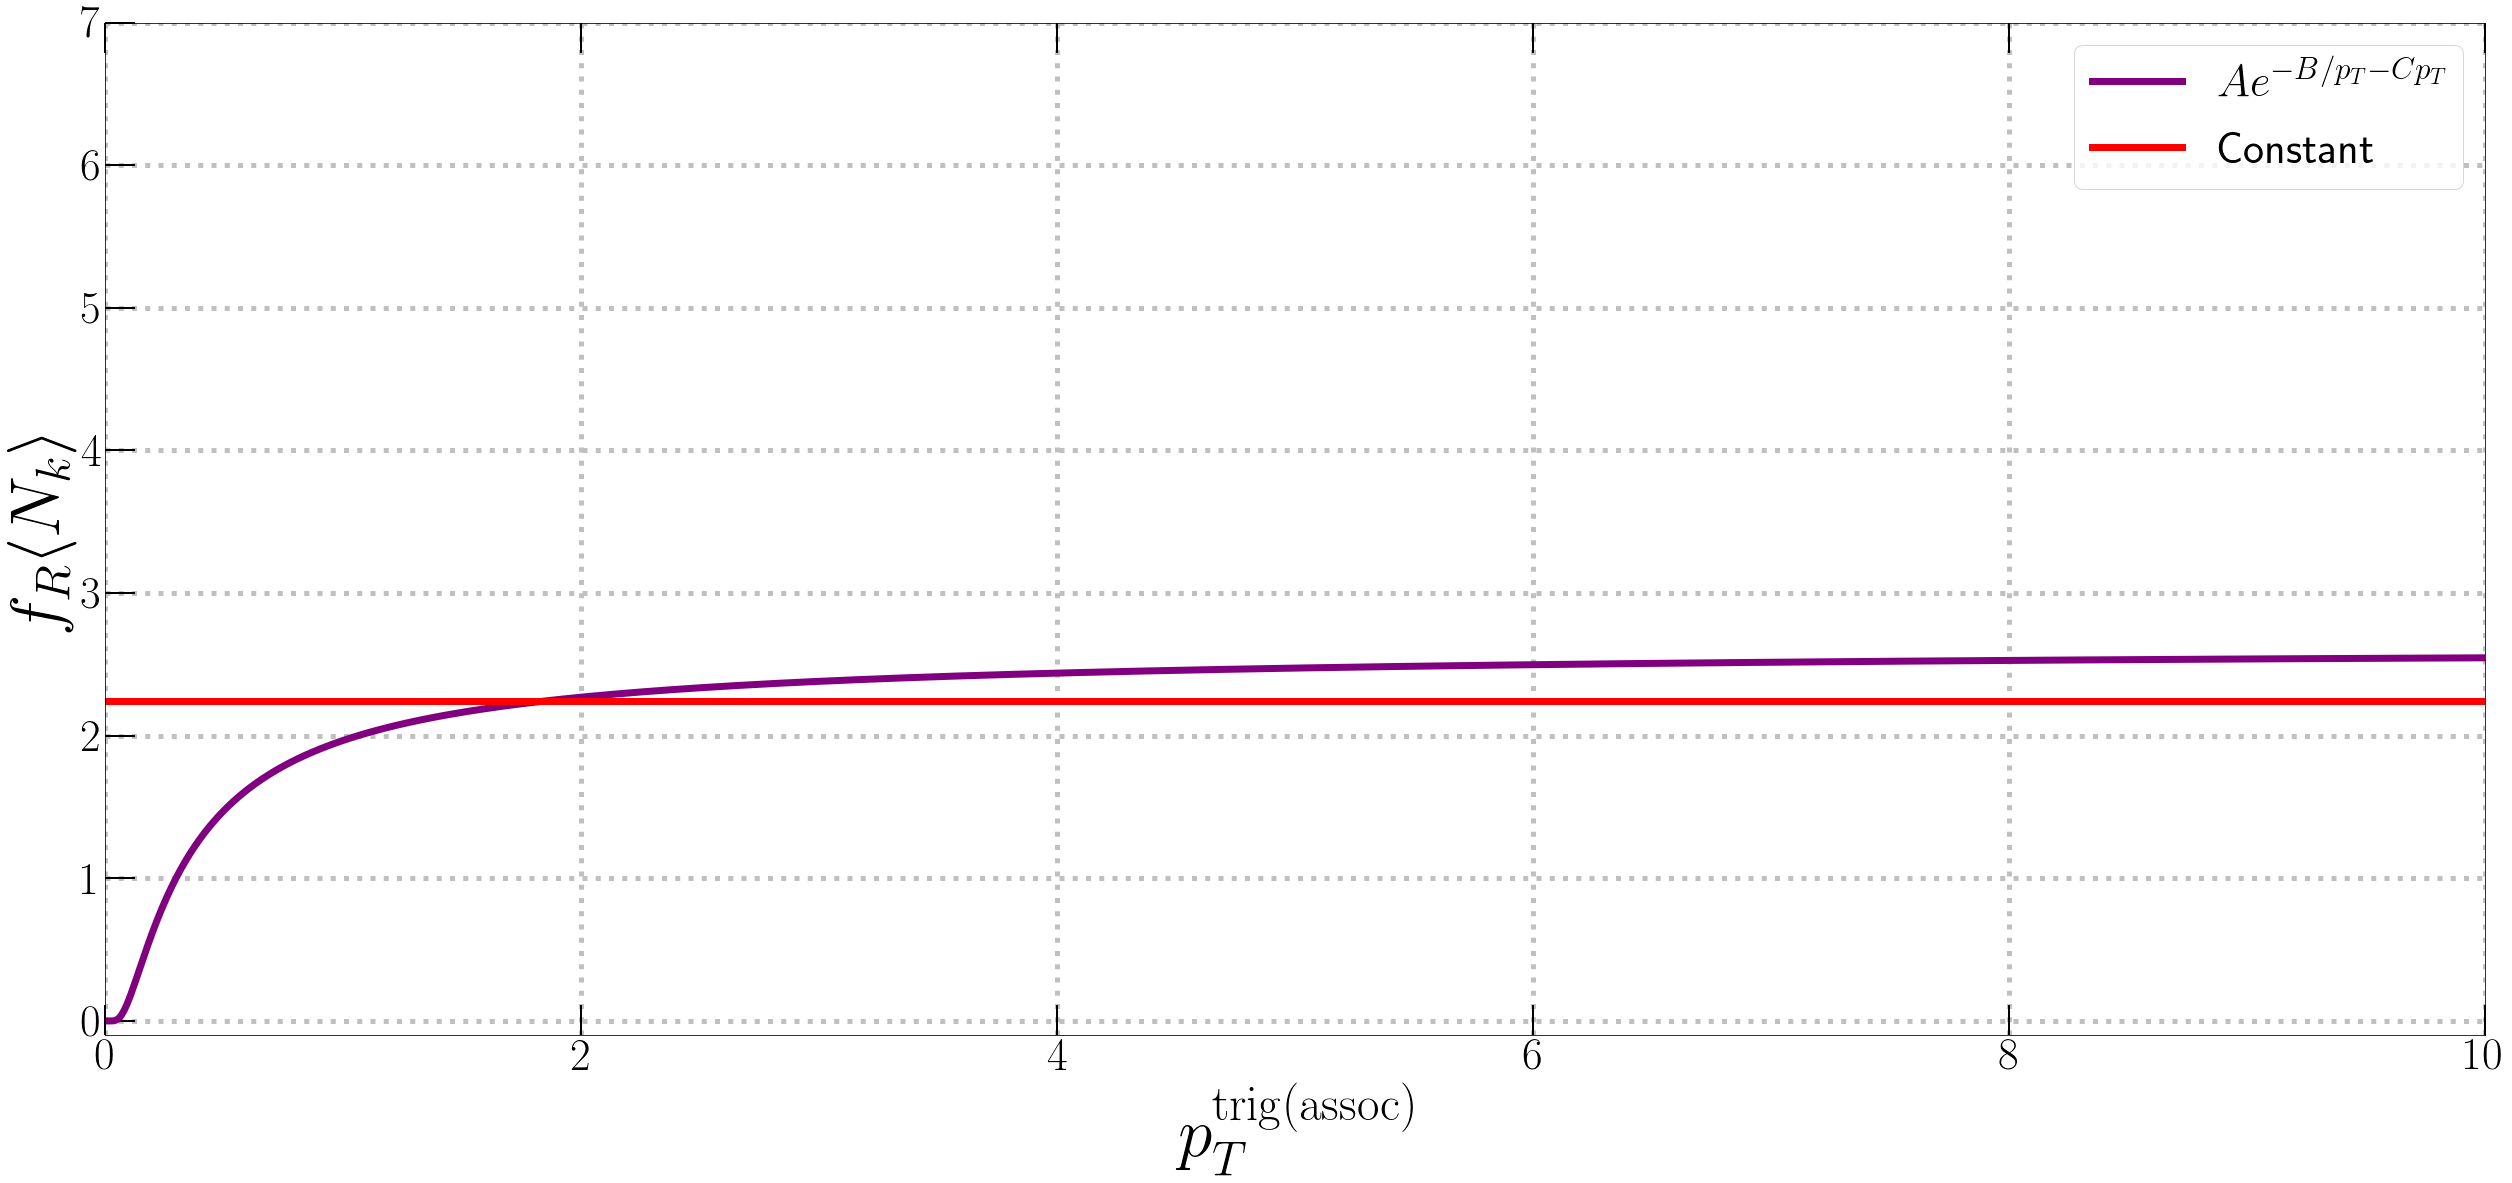
\includegraphics[width=12cm, height=6cm]{./Figures/ptVSnone}
\caption{The $f_R\langle N_k \rangle$ fitting results of $Ae^{-{B} / p_T -C p_{T}}$ form and constant. The purple line is the fitting results of $f_R\langle N_k \rangle = Ae^{-{B} / p_T -C p_{T}}$, and the red line is the fitting result of $f_R\langle N_k \rangle$ as constant. }
\label{figure:ptVSnone}
\end{figure}

According to Fig.\ref{figure:ptVSnone}, two $f_R \langle N_k \rangle$ results only different in the $0.1<p_T<1$GeV range.
This is because, the least square method via the Levenberg-Marquardt algorithm eliminates $e^{-Cp_T}$ term, and the $e^{-B/p_T}$ term only affects the $0.1<p_T<1$GeV range.
However, $0.1<p_T<1$GeV range is not covered in the ALICE data, and the CMS and ATLAS data in the range have high statistical errors.
Consequently, we cannot determine whether there is a $p_T$ dependence of $f_R\langle N_k \rangle$ in the $0.1<p_T<1$GeV range.
Hence, we assume that $f_R\langle N_k \rangle$ is a constant in this paper.


\subsection{pp collisions at 13 and 7 TeV Fitting results}
\label{subsec: pp collisions Fitting results}

We fit the Momentum-Kick model as a least square method to the ALICE and CMS proton-proton collision 13TeV at high-multiplicity\cite{alice, cms}, and we also draw the ATLAS high-multiplicity pp collision results\cite{atlas}.

\begin{figure}[ht]
\centering

\includegraphics[width=18cm, height=3cm]{./Figures/Paper_phiCorr}
\caption{Results for $\Delta \phi$ correlation. All curves are the Momentum-Kick model result, plots are experimental data.
The red color is the result from ALICE, the black is from CMS and the blue is from ATLAS.
For the ALICE and CMS data, we draw the case of $1<p_T<2, 2<p_T<3, 3<p_T<4$, and we also draw $0.1<p_T<1$ case for CMS data. And in ATLAS data, we draw for $0.5<p_T<5$.}
\label{figure:phicorr}
\end{figure}

\begin{figure}[ht]
\centering
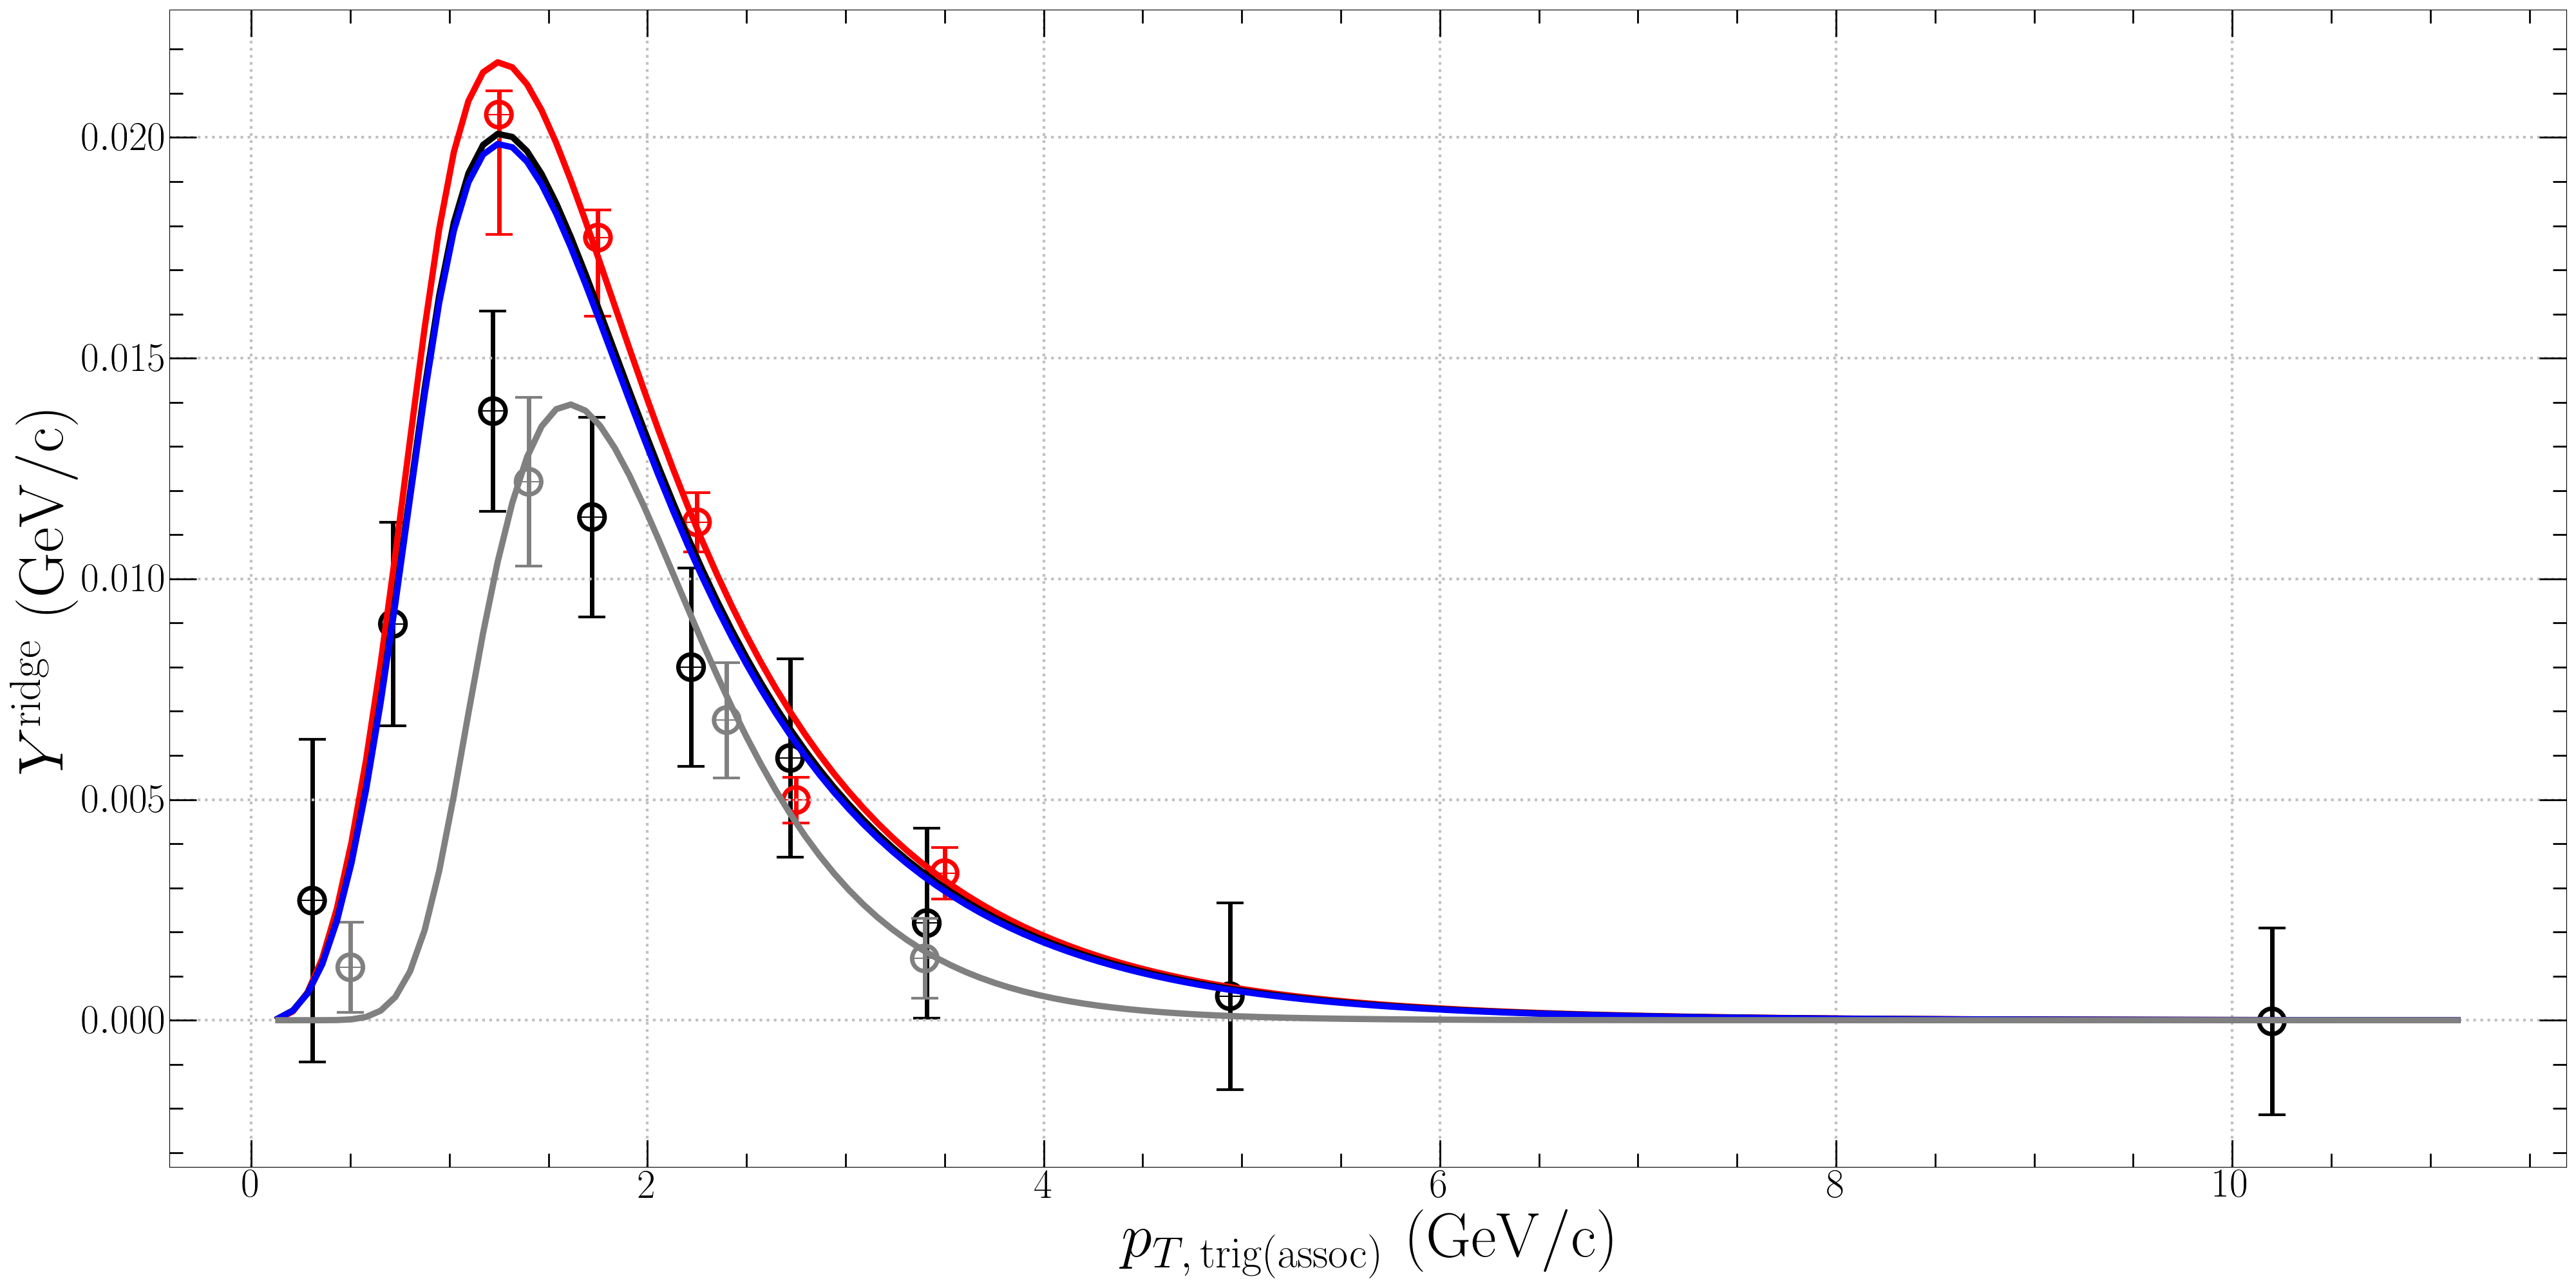
\includegraphics[width=12cm, height=6cm]{./Figures/Paper_pTdis}
\caption{Yield for $p_T$ distribution at ALICE and CMS data. We do not include ATLAS collaboration data, because they don't provide the results for $p_T$ bins.}
\label{figure:pTdis}
\end{figure}

In Fig. \ref{figure:phicorr} and \ref{figure:pTdis}, we draw Momentum-Kick model results and LHC data together.
The solid line is the Momentum-Kick model results, and the circles are the experimental data.
Red color is ALICE data and the Momentum-Kick model results, black is for CMS, and blue is for ATLAS.
In the Fig. \ref{figure:phicorr}, the ATLAS collaboration's data is significantly higher than others.
This is because, they didn't normalize as $p_T$ bin, so I also do not normalize either.
Experimental data is well described via Momentum-Kick model for all $p_T$ ranges.
In Fig. \ref{figure:pTdis}, since partons are kicked as $\textbf{q}$ by jet particles, the theoretical ridge yield must show a peak at $q$.
% However, since $f_R \langle N_k \rangle $ is proportional to ${p_T}^2$, the position of the peak is moved to an area where the $p_T$ is larger. 
As can be seen in Fig.\ref{figure:pTdis}, the peak is made around $p_T=1.2$GeV.
Overall, the Momentum-Kick model can describe well for the $\Delta\phi$ correlation and $p_T$ distribution yield, too.


We are going to compare physical parameters in the ridge component of Momentum-Kick model at STAR AuAu at 200GeV\cite{Wong_1}, CMS PbPb at 2.76TeV\cite{PbPb}, CMS pp 7TeV\cite{cms} and pp at 13TeV, in which ALICE, CMS and ATLAS data are used from reference\cite{alice, cms, atlas}.
Since the number of pp 13 TeV data is sufficient, all parameters of pp at 13 TeV set free parameters.
Due to the insufficient proton-proton data at 7 TeV, we have to find some parameters as physically at 7 TeV.
The reference \cite{Wong_5} and \cite{PbPb} introduced $\langle p_T \rangle$ ratio at the temperature.
Since temperature has $\langle p_T \rangle$ dependence, we can fix temperatrue of pp at 7TeV.
We calculate the temperature of 7 TeV as a ratio of $\langle p_T \rangle$ and it is expressed as:

\begin{equation} \label{equation:Tempratio}
T_{7 \text{Tev}} = T_{13 \text{Tev}} \times \frac{\langle p_T \rangle_{7 \text{TeV}}}{\langle p_T \rangle_{13 \text{TeV}}}
\end{equation}

%마음에 안들지만 일단 패스
% ATLAS:2010jvh -> 7 TeV     ATLAS:2016zkp -> 13 TeV
We get the $\langle p_T \rangle$ data in the ATLAS experiments\cite{ATLAS:2010jvh, ATLAS:2016zkp}.
We set the average $p_T$ as $\langle p_T \rangle _{7 \text{TeV}} = 1.226$ and $\langle p_T \rangle _{13 \text{TeV}} = 1.245$.
Since we aim to study proton-proton collisions at high multiplicity, we utilize the $\langle p_T \rangle$ data within $99.5 < N_{\text{ch}} < 120.5$ and $100.5 < N_{\text{ch}} < 150.5$ for 7 TeV and 13 TeV, respectively.

\begin{equation} \label{equation:7TeVTemp}
T_{7 \text{TeV}} = 1.18 \times \frac{1.226}{1.245} \approx 1.16
\end{equation}

We find free parameters as least square method.
Parameters of ridge component are summarized in Table \ref{table:param}.

\begin{table}[ht]
  \centering
  \begin{tabular}{C{2cm} | C{3cm}  C{4cm}  C{2.5cm}  C{2.5cm}  C{2.5cm}}
   \hline \\[-1 ex]
    & AuAu 200 GeV\cite{Wong_1} & PbPb 2.76 TeV\cite{PbPb} & pp 13 TeV\cite{Hanul} & pp 7 TeV & pp 13 TeV\\ [1 ex] \hline\hline \\[-1.5 ex]
   T (GeV) & 0.5 & 0.6 & 1.54 & 1.16 & 1.18\\[1ex]
   q (GeV) & 1.0 & 0.7 & 2 & 1.33 & 1.00\\ [1ex]
  $f_R \langle N_k \rangle$ & 4 & $20.2e^{-{1.395} / {\langle p_{T}^{\text{trig}} \rangle}-0.207{\langle p_{T}^{\text{trig}} \rangle}}$ & 0.93, 1.37 & 0.99 & 2.24\\[1.5ex]
   \hline
 \end{tabular}
 \caption{All results of the physical parameters in the ridge component of the Momentum-Kick model.}
 \label{table:param}
\end{table}


Since the temperature has center of mass energy dependence, the temperature of proton-proton at 13 TeV is the highest of all the other experiments, which is $+97\%$ higher than PbPb at 2.76 TeV and $+136\%$ higher than AuAu at 200 GeV.
But, it is lower than previous result of ref \cite{Hanul}.
Because they set temperature as ratio of $\langle p_T \rangle$ compare with temperature of AuAu at 200GeV.
However, the number of proton-proton collisions at 13 TeV data has enough to set temperature as a free parameter, and the least-square method find the lower temperature than previous result.

The average of momentum transfer per kick in proton-proton collisions at 13 TeV is about $43\%$ higher than PbPb at 2.76 TeV, but $25\%$ lower than pp at 7 TeV.
because of the higher center of mass energy, $q$ of pp at 13 TeV is higher than PbPb at 2.76 TeV.
However, pp at 13 TeV creates more medium than pp at 7 TeV.
Because of the jet kicking more mediums in the pp at 13 TeV, the average momentum transfer per kick goes lower.
Hence, the pp at 13 TeV of $q$ is lower than pp at 7 TeV.

The last parameter, $f_R \langle N_k \rangle$, is lower in the pp collisions than heavy-ion collisions.
Because the pp collisions make the small system, and the heavy-ion collisions are not.
Also, the $f_R \langle N_k \rangle$ of 13 TeV is larger than the 7 TeV, because the higher center of mass energy creates more medium.
Fig.\ref{figure:frnk} is a graph compared with references\cite{Wong_1, PbPb, Hanul}.


\begin{figure}[ht]
  \centering
  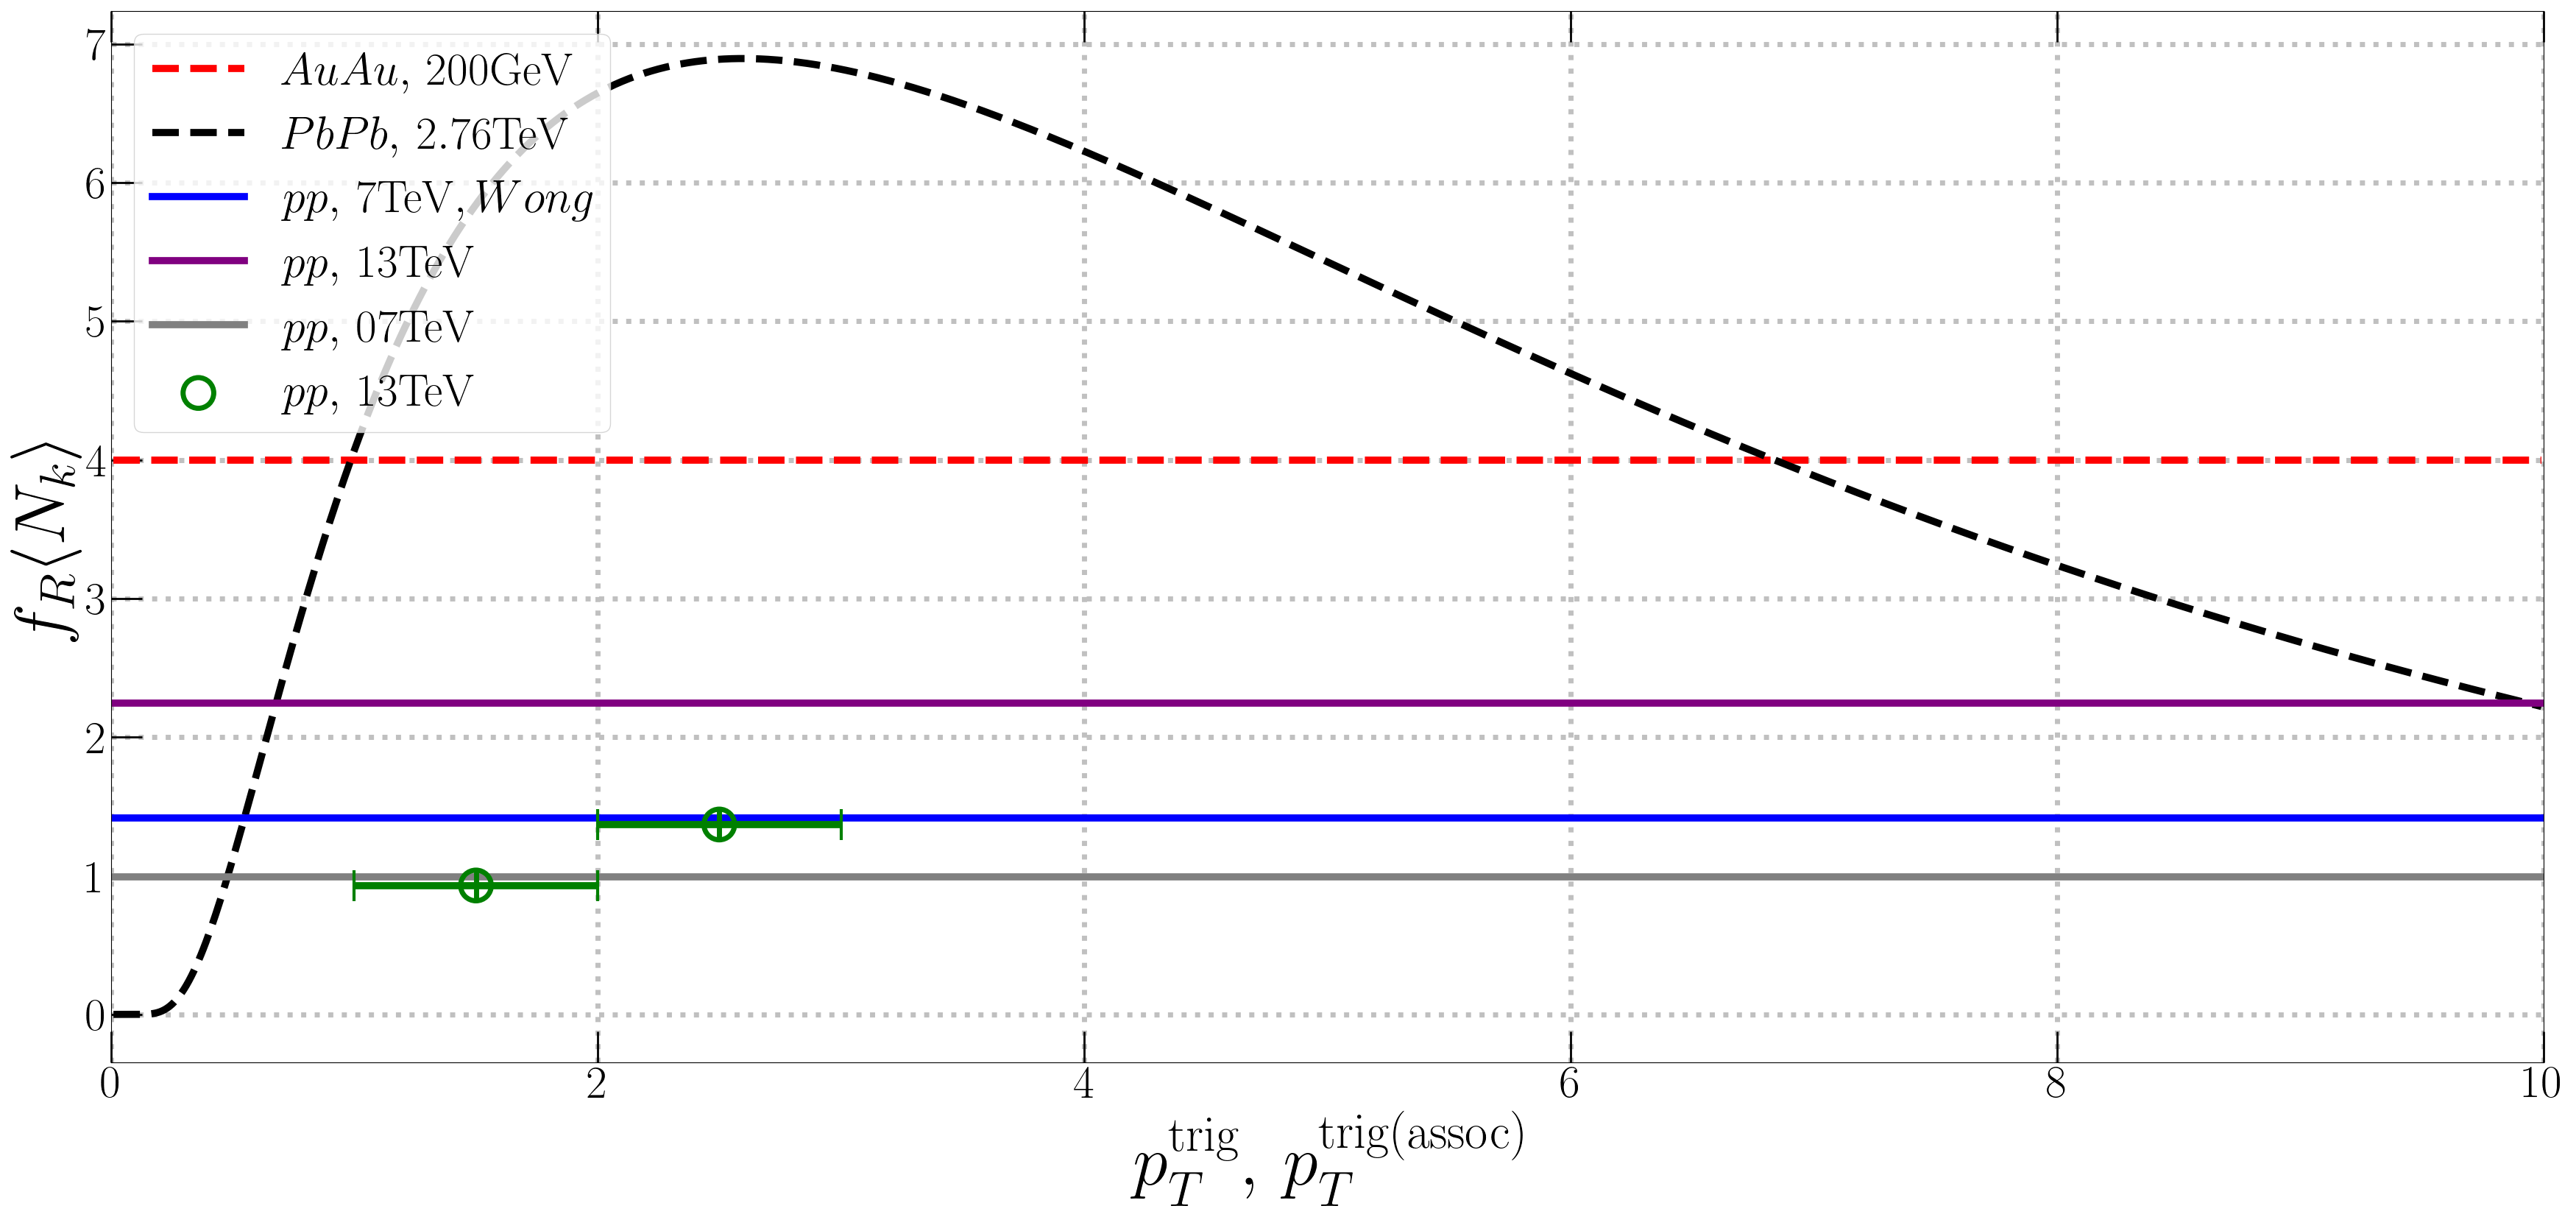
\includegraphics[width=12cm, height=6cm]{./Figures/Paper_frnk}
  \caption{The shape of $f_R \left\langle N_k \right\rangle$ in AuAu at 200GeV, PbPb at 2.76TeV and pp at 13TeV for $p_{T}^{\text{trig}}$.
  The dotted lines are the Momentum-Kick model's results of heavy-ion collisions, and the solid lines are the cases of proton-proton collisions.
  The red color is AuAu at 200 GeV\cite{Wong_1} and the black color is PbPb at 2.76 TeV\cite{PbPb}.
  The blue color is previous the Momentum-Kick model of pp at 7 TeV result\cite{Wong_5}, and the green plots are the results of the reference\cite{Hanul}.
  And the others, the purple and grey colors, are the finding of this study for the pp at 13 TeV and 7 TeV, respectively.
  }
  \label{figure:frnk}
\end{figure}

The PbPb at 2.76 TeV and pp at 13 TeV show the results in several bins for $p_T^{\text{trig}}$, and the range of $p_T^{\text{assoc}}$ is only split equal to $p_T^{\text{trig}}$ in the pp at 13TeV.
However, we can compare the trend.

In the case of AuAu collision at 200GeV, since it has low energy, $f_R \langle N_k \rangle$ does not have $p_T$ dependence.
PbPb at 2.76 TeV has high energy and creates high medium density, $f_R$ has exponentially increase and $\langle N_k \rangle$ has exponentially decrease as $\langle p_T^{\text{trig}} \rangle$.
This is because, the particles, which are the high-range of $p_T$, can survive easily, but the number of kicked medium partons gets lower.
Hence, the reference\cite{PbPb} decided $f_R \langle N_k \rangle$, which has $\langle p_T^{\text{trig}} \rangle$ dependence.
However, because of lower density in pp collision, we set $f_R \langle N_k \rangle$ as constant due to mention earlier\ref{subsec: pT depnedence}.

\subsection{How about the other multiplicity results?}
\label{subsec: How about the other multiplicity results?}

We already know that the near-side ridge structure appears in the high multiplicity proton-proton collisions, which is well described as the Momentum-Kick model.
So, we have to check the other multiplicity, like the low multiplicity.
Firstly, $q$ is same as pp at 13 TeV in the high multiplicity.
The CMS and ATLAS collaboration provide $\Delta \phi$ correlation in the various multiplicity, but the CMS collaboration data have very high fluctuation, I use only ATLAS data.

% The reference \cite{Wong_5} and \cite{PbPb} introduced $\langle p_T \rangle$ ratio at the temperature.
As previously stated, we set the temperature in the pp collisions at 7 TeV as $\langle p_T \rangle$ ratio.
Since the $\langle p_T \rangle$ is getting higher at the higher multiplicity\cite{ATLAS:2016zkp}, the temperature has multiplicity dependence.
Hence, we also introduced $\langle p_T \rangle$ ratio at the $T$ in other multiplicities, based on the temperature of high multiplicity, which is expressed as follows:

% 아래 식은 무리수인가...?
\begin{equation} \label{equation:variousmulti}
  T_{\text{other multiplicities}} = T_{\text{high multiplicity}} \times \frac{\langle p_T \rangle_{\text{other multiplicities}}}{\langle p_T \rangle_{\text{high multiplicity}}}
\end{equation}

%흠 이부분 어쩌지%
Also, following figure \ref{figure:frnk_multi} is integrated near-side yields, which is the graph of ridge yield dependence of multiplicity.
Since we already know that $f_R \langle N_k \rangle$ describes the number of particles, $f_R \langle N_k \rangle$ should explain integrated near-side yields.
Hence, we introduce multiplicity dependence in the $f_R \langle N_k \rangle$ as linearly and we fit the $f_R \langle N_k \rangle$ in the integrated near-side yields.

\begin{figure}[ht]
  \centering
  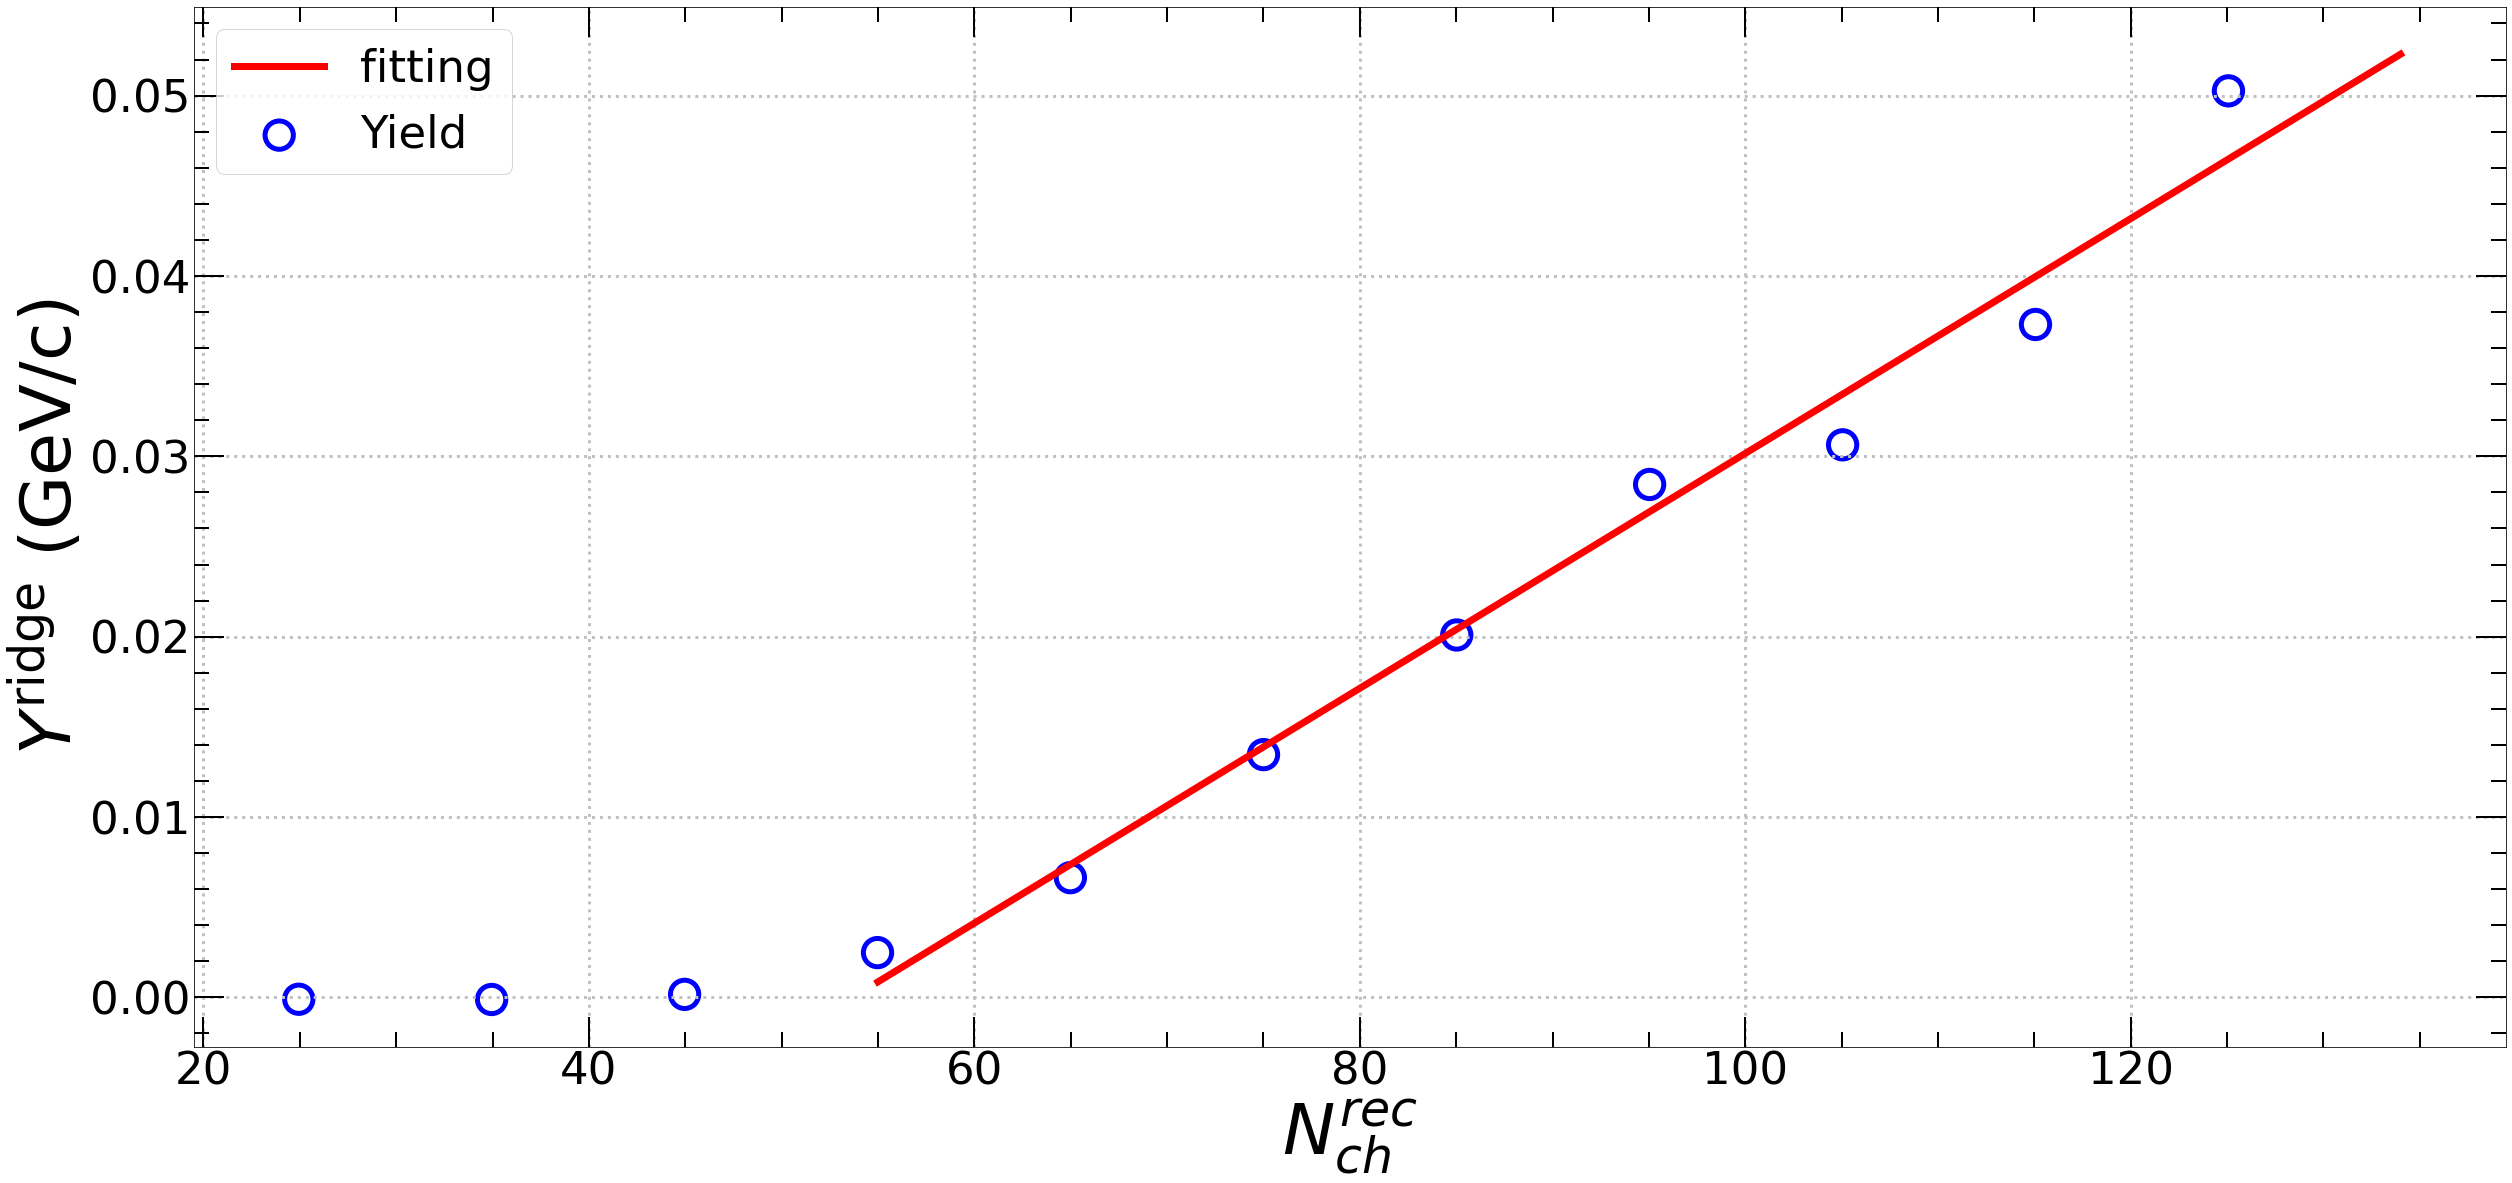
\includegraphics[width=12cm, height=6cm]{./Figures/Yield_Fitting.png}
  \caption{Integrated long-range near-side yield vs multiplicity in proton-proton collisions at 13 TeV.
  The ATLAS experimental results are shown in blue plots\cite{atlas}, and a linearly fitted line for these blue plots is represented by the red line.
  And the fitting result is used as $f_R \langle N_k \rangle$.
  }
  \label{figure:frnk_multi}
\end{figure}

% 씁 이부분 어떻게 써야 하려나...
Since linear function can describe the ridge yields well in the $50\leq N_{\text{ch}}^{\text{rec}}$, we set $f_R \langle N_k \rangle$ as $A(B+C N_{\text{ch}}^{\text{rec}})$, $A$ is normalization constant, $B$ and $C$ is fitted value as we mentioned earliear.
Also, we think that the jets get the same energy within the same center-of-mass energy systems, so we set $q$ the same as the high multiplicity result.
Therefore, the parameter '$A$', which is in the $f_R \langle N_k \rangle$, is the only free parameter.
The table\ref{table:variousmulti} and the figure\ref{figure:variousmulti} are the fitting results of proton-proton collisions at 13 TeV in the various multiplicities.

\begin{table}[ht]
  \renewcommand{\arraystretch}{1.5}
  \begin{tabular}{C{3cm} | C{1.5cm} | C{1.5cm} | C{6cm}}
  \hline
  $N_{\text{ch}}^{\text{rec}}$         &  $q$   &   $T$   & $f_R\langle N_k \rangle$ \\ \hline\hline
  $50\leq N_{\text{ch}}^{\text{rec}}<60$   &        & $1.096$ & $0.220(-35+0.65\langle N_{\text{ch}}^{\text{rec}}\rangle)\times10^{-3}$ \\ \cline{1-1} \cline{3-4} 
  $60\leq N_{\text{ch}}^{\text{rec}}<70$   &        & $1.117$ & $0.292(-35+0.65\langle N_{\text{ch}}^{\text{rec}}\rangle)\times10^{-3}$ \\ \cline{1-1} \cline{3-4} 
  $70\leq N_{\text{ch}}^{\text{rec}}<80$   &        & $1.138$ & $0.308(-35+0.65\langle N_{\text{ch}}^{\text{rec}}\rangle)\times10^{-3}$ \\ \cline{1-1} \cline{3-4} 
  $80\leq N_{\text{ch}}^{\text{rec}}<90$   &        & $1.157$ & $0.357(-35+0.65\langle N_{\text{ch}}^{\text{rec}}\rangle)\times10^{-3}$ \\ \cline{1-1} \cline{3-4} 
  $90\leq N_{\text{ch}}^{\text{rec}}<100$  & $1.00$ & $1.172$ & $0.422(-35+0.65\langle N_{\text{ch}}^{\text{rec}}\rangle)\times10^{-3}$ \\ \cline{1-1} \cline{3-4} 
  $100\leq N_{\text{ch}}^{\text{rec}}<110$ &        & $1.188$ & $0.359(-35+0.65\langle N_{\text{ch}}^{\text{rec}}\rangle)\times10^{-3}$ \\ \cline{1-1} \cline{3-4} 
  $110\leq N_{\text{ch}}^{\text{rec}}<120$ &        & $1.212$ & $0.429(-35+0.65\langle N_{\text{ch}}^{\text{rec}}\rangle)\times10^{-3}$ \\ \cline{1-1} \cline{3-4} 
  $120\leq N_{\text{ch}}^{\text{rec}}<130$ &        & $1.229$ & $0.507(-35+0.65\langle N_{\text{ch}}^{\text{rec}}\rangle)\times10^{-3}$ \\ \cline{1-1} \cline{3-4} 
  $130\leq N_{\text{ch}}^{\text{rec}}$     &        & $1.233$ & $0.443(-35+0.65\langle N_{\text{ch}}^{\text{rec}}\rangle)\times10^{-3}$ \\ \hline
  \end{tabular}
  \caption{The results of the physical parameters in the various multiplicities.
  $\langle N_{\text{ch}}^{\text{rec}}\rangle$ means the average of $N_{\text{ch}}^{\text{rec}}$.
  We set $\langle N_{\text{ch}}^{\text{rec}}\rangle$ as the half of each multiplicity range.
  }
  \label{table:variousmulti}
\end{table}

\begin{figure}[ht]
\centering
\includegraphics[width=15cm, height=15cm]{./Figures/rezero_atlas_Nk.png}
\caption{$\Delta \phi$ correlation results in various multiplicity.
The plots are experimental data, and the solid lines are the Momentum-Kick model results.
}
\label{figure:variousmulti}
\end{figure}

%여기다 무엇을 써야 할까나...?%


\section*{CONCLUSIONS}
\label{sec:Conclusion}


We have analyzed the long-range near-side proton-proton collisions at $\sqrt{s_\text{NN}}=13$TeV in ALICE, CMS and ATLAS collaborations\cite{alice, cms, atlas}, $\sqrt{s_\text{NN}}=7$TeV in CMS data\cite{cms}, and the various multiplicity in the ATLAS collaboration\cite{atlas}.

%high multiplicity 13 TeV, 7 TeV 결과%
Firstly, the Momentum-Kick model can describe well the high multiplicity proton-proton collisions.
Since the small systems have less flow effect than heavy-ion collision, we expect that the Momentum-Kick model is applicable in this case.
We apply the Momentum-Kick model in the high multiplicity pp collision at 13 TeV data from all 3 collaborations and 7 TeV data from the CMS collaboration. 
As a result, we obtain $T=1.18$ GeV, $q=1.00$ GeV, $f_R\left\langle N_k\right\rangle = 2.24$ in 13 TeV, and $T=1.16$ GeV, $q=1.33$ GeV, $f_R\left\langle N_k\right\rangle = 0.99$ in 7 TeV.
Because of higher energy, the medium temperature of 13 TeV is 97\% higher, and the temperature of 7 TeV is 93\% higher than PbPb collision at 2.76TeV.
Also, because the medium from pp collision has less density than heavy-ion collisions, the jet particles kick the number of medium partons less than PbPb collision.
Therefore, the average momentum transfer per kicked medium partons is 43\% higher in 13 TeV and 90\% higher in 7 TeV than PbPb collision at 2.76TeV.
Furthermore, the $f_R\left\langle N_k\right\rangle$ results of both center-of-mass energy systems of proton-proton collisions are less than PbPb collisions at 2.76TeV.
Moreover, the $f_R\left\langle N_k\right\rangle$ at 7 TeV is lower than at 13 TeV, which is shown that lower center-of-mass energy creates less mediums.


%various multiplicity 결과%
Secondly, the Momentum-Kick model with introduced multiplicity dependence in $f_R\left\langle N_k\right\rangle$ can also apply well in the various multiplicities.




% We also introduce $p_T$ dependence on $f_R\left\langle N_k\right\rangle$ as in the reference\cite{PbPb}.
% Since high density is created in PbPb at 2.76TeV collision, jet particles kick many of initial medium particles as $\textbf{q}$.
% Therefore, many of final particles, which is middle range of $p_T$, are created.
% As a result, $f_R \langle N_k \rangle$ in PbPb collision has a maximum value at mid-range of $p_T$.
% The particles that the high range of $p_T$ can survive easily in the proton-proton collision, it has the same as PbPb collisions.
% However, since pp collision at 13TeV makes lower density than PbPb collisions, the number of kicked medium partons is irrelevant to $p_T$.

Furthermore, we expect the Momentum-Kick model can well describe other diverse data.
Therefore, we will try to explain other data, like various multiplicity and center of mass energy, via the Momentum-Kick model.
\bibliography{Bibliography}

\end{document}
